\documentclass[12pt,a4paper]{article}

\usepackage{epcc}
\usepackage{graphicx}
\usepackage{hyperref}


\begin{document}

\title{Coursework for Programming Skills}
\author{Nikilesh Balakrishnan\\
        Mark Florisson\\
        Dante Gama Dessavre\\
        He Li\\
        Shun Liang\\
        Sinan Shi}
\date{\today}

\makeEPCCtitle

\thispagestyle{empty}

\newpage

\pagenumbering{roman}

\tableofcontents

\newpage

\pagenumbering{arabic}

\section{Introduction}

The objective of this coursework is to implement a sequential version of a two-dimensional predator-prey model with spatial diffusion. The governing equations for this problem are:

\begin{equation}
\frac{\partial H}{\partial t}=rH-aHP+k\left(\frac{\partial^2 H}{\partial^2 x}+\frac{\partial^2 H}{\partial^2 y}\right)\\
\end{equation}

\begin{equation}
\frac{\partial P}{\partial t}=bHP-mP+l\left(\frac{\partial^2 P}{\partial^2 x}+\frac{\partial^2 P}{\partial^2 y}\right)\\
\end{equation}

where $H$ is the density of hares (prey) and $P$ the density of pumas (predators). $r$ is the intrinsic rate of prey population increase, $a$ the predation rate coefficient, $b$ the reproduction rate of predators per one prey eaten and m the predator mortality rate. $k$ and $l$ are the diffusion rates for the two species.

Even though this is not a simple problem to analyze from a theoretical perspective, a lot can be learned from a simplification of it. If we assume that both initial densities of hares and pumas are uniform, then the diffusion term in equations (1) and (2) has no effect, so the problem is reduced to:

\begin{equation}
\frac{\partial H}{\partial t}=rH-aHP
\end{equation}

\begin{equation}
\frac{\partial P}{\partial t}=bHP-mP
\end{equation}

These are the Lotka-Volterra equations for prey-predator systems. After doing some mathematical analysis using the parameters provided in the handout, there are two stable points. The first is (0,0) which is a saddle point attracting vectors in the y axis and repelling them in the x axis. The second is (3,2) which is a neutrally stable point, which means that cycles are formed around this point with a counter clockwise direction. The vector field and a sample cycle is shown in Figure 1. All this analysis proved useful during testing of the code.  %The vector field characterizing the solutions to equations (3) and (4) using the parameters given in the coursework handout can be seen in Figure 1. 

%\begin{figure}[hb]
%    \centering
%    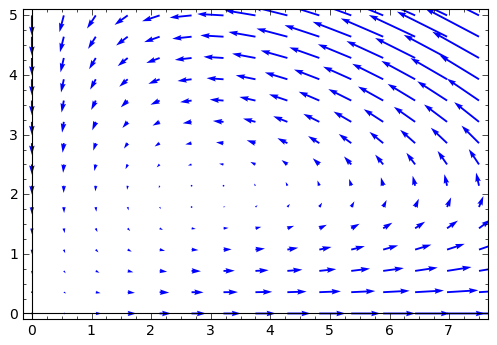
\includegraphics[scale=0.75]{images/sage0.png}
%    \caption{Vector field of equation 2}
%\end{figure}

\clearpage


\begin{figure}[hb]
    \centering
    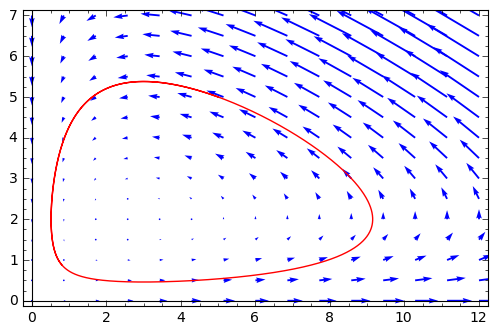
\includegraphics[scale=0.75]{images/sage2.png}
    \caption{Vector field of equation 2}
\end{figure}



\section{Planning and Task Division}

The Systems Modeling Language standard was utilized for designing the software, since it is a modification of UML that is more suitable for non object oriented software. 

The block diagram of the system can be seen in Figure 2. There are four main blocks or components: an input/output (I/O) library, the partial differential equation (PDE) computation kernel, the main simulator and a unit testing component.

The I/O library (Figure 3) consists of two main elements. Firstly there is the read function which accepts the matrices that correspond to the island, hares and pumas. The second one is the write function that handles the creation of the \texttt{ppm} files that contain the output for visualization. It also contains two auxiliary components alongside an error handling element.

The PDE component (Figure 4) consists mainly of the compute function that implements the approximation formula for estimating the solution to the partial differential equations that model the problem.

The main component takes care of parsing the user input and printing the usage, but its primary purpose is to utilize the I/O and PDE components in order to solve the problem. The internal block diagram can be seen in Figure 5, which contains a flow diagram of how the main component was designed.

Finally, the figure 6 details the unit testing component, whose main element is similar to the one in the main program's component, but with additional automated testing elements, so it doesn't need to parse the user input.


\begin{figure}[hb]
    \centering
    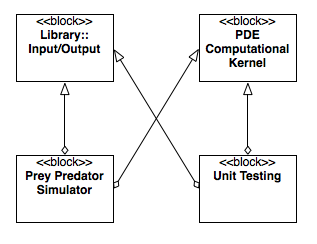
\includegraphics[scale=0.6]{images/blockdesign.png}
    \caption{Vector field of equation 2}
\end{figure}

\begin{figure}[hb]
    \centering
    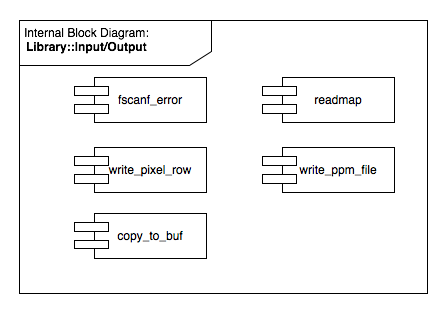
\includegraphics[scale=0.6]{images/bd1.png}
    \caption{Vector field of equation 2}
\end{figure}

\begin{figure}[hb]
    \centering
    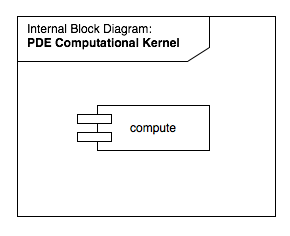
\includegraphics[scale=0.6]{images/bd2.png}
    \caption{Vector field of equation 2}
\end{figure}

\begin{figure}[hb]
    \centering
    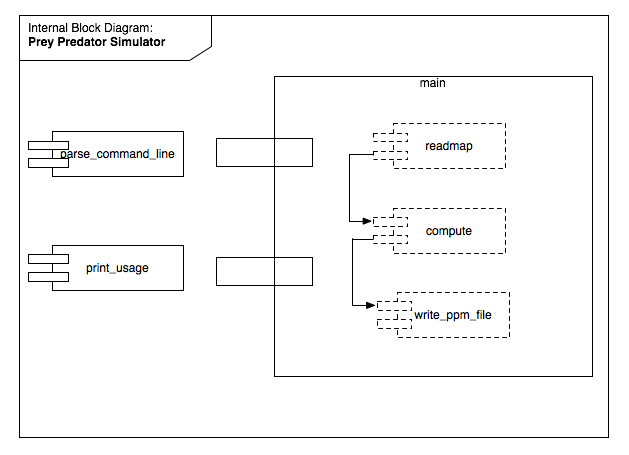
\includegraphics[scale=0.6]{images/bd3.png}
    \caption{Vector field of equation 2}
\end{figure}

\begin{figure}[hb]
    \centering
    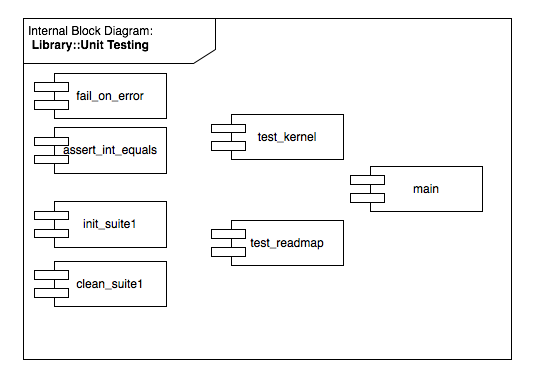
\includegraphics[scale=0.6]{images/bd4.png}
    \caption{Vector field of equation 2}
\end{figure}

\clearpage


\subsection{Task Division}

Work on the components was divided as follows:

\begin{tabular}{ | l || l | }
    \hline
    Input/Output  & Mark and Nikilesh \\
    \hline
    Computational Kernel & Shun and He \\
    \hline
    Error Testing & Sinan and Dante \\
    \hline
\end{tabular}

Work on performance analysis and deployment was mainly shared between all the members of the team.

%\begin{figure}
%
%\begin{center}
%\resizebox{0.30\hsize}{!}{
\includegraphics{logos/eucrest}}
%\end{center}
%
%\caption{The University Crest}
%\label{fig:eucrest}
%
%\end{figure}

\section{Implementation and documenting}

The implementation was made in the C language, with an additional Matlab program to generate the test cases. We used a distributed revision control software called Git, with a central repository located in \url{https://github.com/markflorisson88/puma}.

\subsection{Data Structures}

The map was modeled as a grid of land/water cells and implemented as two-dimensional C array. The population densities of predators and preys are modeled in the same way. The \texttt{Real} type defined as a macro represents the value in the density grids, so different floating point precision  can be specified in compile time. 

A struct, \texttt{EquationVariables}, was created as a wrapper for the parameters of the equations.

\subsection{Computational Kernel}

The (PDE) computational kernel consists primarily of the \texttt{compute} function. The parameters of the function are: the predator and prey density grids, the grid of land/water cells and a pointer to a \texttt{EquationVariables} struct that contains the parameters of the equations.

Two 2002 $\times$ 2002 size global grids are used temporarily to store the value of new predator and prey densities. For each land cell in the density grid the values of the adjacent cells are read, which then are used for the calculation of the new values (along with the equation parameters). On the other side water cells are ignored. After the new density is computed the value is stored into the temporary density grid. Once all new densities are computed, the new values are assigned back to the original predator and prey density grids from the temporary grids.

The computation is performed until the time, given by the user, is reached.

%The computational kernel is invoked in the main program $N$ times, where $N$ is specified by the user in command line.

\subsection{Data Input and Output}

The readmap function is used to read in a two dimensional array of integers. The first line specifies the length of the columns and rows, and the subsequent lines specify the values for the elements in the array. This is useful to read in files that specify the landscape.

\subsection{Error Handling}

The file \texttt{include/\_errors.h} has the project-specific \emph{errnos}. These can be returned from a function to indicate which error occurred. The caller can then act based on this value, or retrieve and print an error message associated with that errno (\texttt{puma\_strerror}). If the error was caused by the OS, the functions return \texttt{PUMA\_OSERROR}, for which message retrieval is delegated to the function \texttt{strerror}.

Also a simple logging utility was implemented that can write debug and error messages. The debug messages will be enabled when the code is compiled with the \texttt{-DDEBUG} flag.


%There is a file \texttt{include/_errors.h} that has project-specific errnos. These can be returned
%from a function to indicate which error occurred. The caller can then act based on this value, or
%retrieve and print an error message associated with that errno (\texttt{puma_strerror}). If the error
%was caused by the OS, the functions return \texttt{PUMA_OSERROR}, for which message retrieval is delegated
%to the function \texttt{strerror}.

%1. Wrote the Makefile scripts.

%2. Implemented a simple logging utility that can write debug and error messages. The debug messages will be enabled when the code is compiled with the -DDEBUG flag.
%3. Implemented the output to .ppm file functionality.
%4. Wrote function to parse user input.
%5. Wrote perl script to compare C program results with results produce by the Matlab program.


\section{Testing}

\subsection{Unit Testing}

%Unit testing is to test the program by testing its individual module or parts. The object of unit testing is to isolate each part of the program and show that the individual parts are correct%\cite{unittest}.

The testing framework CUnit was used for performing unit tests. The basic functionality of the framework was utilized, which provides a non-interactive output to \texttt{stdout}. The basic structure of CUnit is a hierarchy of test registries, suites, and test cases, which are initialized before the test, and cleaned up afterwards.

%The test will be run only in Basic interface with non-interactive output to sdout . 

%We do our unit testing with CUnit as unit testing framework. CUnit provide the user a library to build their test structures. 
%. Those parts must be initialized before the test and clean up registry after the test.


\subsubsection{Input and Output Testing}

Input and Output were tested in two different ways. The output was tested manually since it was easy to provide a data file and visually check if the result is the expected one. 

The input was tested using the CUnit framework by reading the identity matrix and checking the resulting matrix in the program. 

%The I/O reading was tested by writing a small amount of synthetic data to a file and then reading that in and verifying that the data is correct. For the data we chose the identity matrix, which is easy to verify.

%3. Implemented the output to .ppm file functionality.

\subsubsection{Computational Kernel Testing}

%TODO: Add final results of unit testing and complaining of delta_t=0.4 >:( 

For testing the computational kernel two techniques were used. The first one was CUnit, utilizing results from a simple MATLAB program as test cases. Only the values of the hare density were checked for simplicity, and the fact that a correct answer there pretty much guarantees a correct answer in the pumas density. A method, called \texttt{CU\_ASSERT\_DOUBLE\_EQUAL}, was added to verify the solutions, since the native CUnit functions are limited with regards to identifying the errors (they just print that there is an error, but not what error or where). The tolerance for the tests was $1 \times 10^{-5}$.

There are a couple notable aspects about performing this tests, and after doing the mathematical analysis of the equations, the results started to make sense. 

First, the results of the MATLAB code were verified thanks to the analysis presented in the introduction of the report.

When time steps of size 0.4 were used, the software never passed the the test cases. The results when using that value can be seen in Figure 7. But when the time step was changed to 0.004 (which in principle should produce more accurate results), the test were passed satisfactorily. 


%To verify the kernel code is equivalent to verify function compute, we generate 3 small scale matlab simulation testing cases to check the solution of kernel code. According to matlab simulation, a set of final results, density of puma and hare, will be provided. We run the function compute in some certain iteration, same as the simulation or the instruction of analysis. And check the value on each grid of map if they are what we expected. For simplicity, we only check the value of density of hares, since the density of puma is dependent of hares. We use CU_ASSERT_DOUBLE_ EQUAL function in CUnit to verify the solutions. Since CUnit function will not return the proper error information (just print the error command line). We have made some functions to return the error value and true value as well and, we set tolerance equal to 1.0e-5.

%To verify the kernel code is equivalent to verify function compute. Behaviour analysis and matlab simulation will be done before the kernel testing. According to behaviour analysis or matlab simulation, a set of final results, density of puma and hare, will be provided. We run the function compute in some certain iteration, same as the simulation or the instruction of analysis. And check the value on each grid of map if they are what we expected. For simplicity, we only check the value of density of hares, since the density of puma is dependent of hares. %We use CU_ASSERT_DOUBLE_ EQUAL function in CUnit to verify the solutions. We can set the tolerance is equal to $1.0e-5$. 


\subsection{Script Testing}

%TODO: Add explanation of behaviour of result

In order to verify the behaviour of the results in the program, particularly important given the failed test cases when using 0.4 as step size, a perl script to compare the C program results with results produce by the Matlab program at various time steps of the algorithm. 

A graph of the results of the MATLAB algorithm can be seen in Figure 7 (once again using uniform starting densities and the handout parameters). Contrary to the results predicted by the analysis, the results diverged, and if a big final time parameter was used, the results wen to infinity (throwing a \texttt{NaN} result). A similar behaviour was observed in the C program.

On the other hand two results of the C program, using time steps of 0.004, can be seen in Figure 8. Here the result was the stable cycle that was expected, and it was the same result for both MATLAB and C code.

Also there was an introduction to this kind of problems in a recent lecture Parallel Numerical Algorithms, that talked about how this algorithms can fail due to the choice of time step. That seems to be the case in this result, the use of time steps of 0.4 produces a divergent result that is due to error in the algorithm and not an actual approximation to the solution. Both the C and MATLAB codes produced wrong results, and the fact that the wrong results they produced were different actually told us nothing about the correctness or the program. It was when using an adequate time step that both programs had a result similar to what we had expected, and since they coincided when dealing with these correct result one can conclude that the program passes the tests that it should once adequate parameters are utilized.

\begin{figure}[hb]
    \centering
    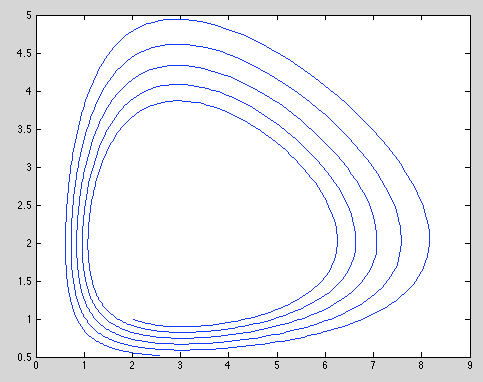
\includegraphics[scale=0.5]{images/diverge.png}
    \caption{Vector field of equation 2}
\end{figure}




\begin{figure}[hb]
    \centering
    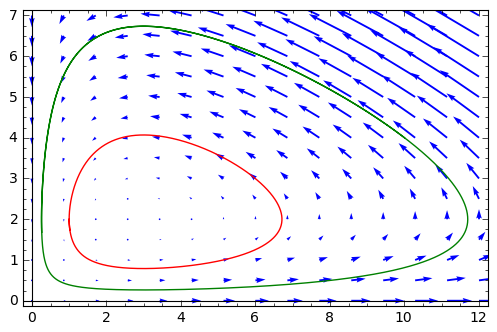
\includegraphics[scale=0.75]{images/sage1.png}
    \caption{Vector field of equation 2}
\end{figure}

\clearpage

\subsection{Stress Testing}

Stress testing was the final stage of the testing phase of development. It was performed using extreme and incorrect parameters. The stress test cases included:

\begin{enumerate}

\item Bad coefficient values (0 or negative) in command line arguments;
\item Bad time step value (negative or greater than 1) in command line arguments;
\item Bad write out interval (negative or greater than the number of iterations) in command line arguments;
\item Input file which is larger than the allowable size (2000 $\times$ 2000);
\item Input file dataset with the max allowable size (2000 $\times$ 2000);
\item Input file contains header only and no map cells;
\item Input file contains nothing;
\item Input file contains less number of cells than the number specified in its header;
\item Input file contains more number of cells than the number specified in its header;

\end{enumerate}

For the stress test cases 1 to 8, the program exits outputting a relevant error message. For case 9, the program runs with the subset of the map in the input file with the size specified in the file header.

\section{Deployment and Performance Analysis}

\subsection{Performance testing} 


The first step of the performance testing was utilizing different compiler optimization flags, which are shown in the next table:

\begin{tabular}{ | l || l | }
    \hline
    gcc optimization flags:  & \texttt{-O1, -O2, -O3} \\
    \hline
    Running environment:  & Quad Core Intel i7 Computer \\
    \hline
\end{tabular}

Figure 9 shows the running time of different optimization options and landscape sizes, utilizing single precision. The most notable aspect is the difference between the code compiled with no flags with the one compiled with the \texttt{-O1} flag. The optimizations provided by this level made the performance behaviour with respect to matrix size to be a lot more linear than the unoptimized code (which shows a near exponential growth), which wasn't a result that was expected beforehand. On the other hand, the similar behaviour between the  \texttt{-O1, -O2} and  \texttt{-O3} levels was to be expected given the simplicity of the code, and the fact that the data alignment optimizations provided by the \texttt{-O2} flags don't help much since the data was already nicely aligned to start with.

Figure 10 shows that when double precision was used, there werw no significant difference in either behaviour nor execution times when compared to single precision. What this shows it shows is that the CPU it was executed on was equally capable of double precision floating point operations ad single precision ones and that the compiler optimizations had the same effects in both cases.


\begin{figure}[hb]
    \centering
    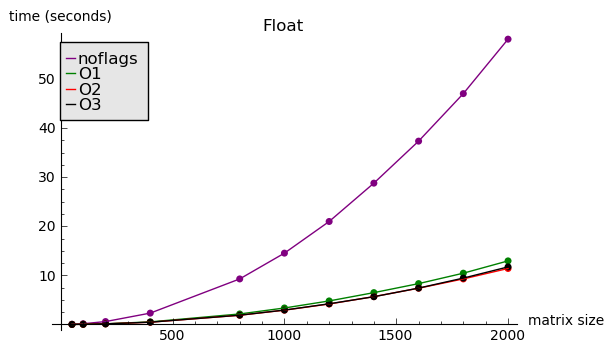
\includegraphics[scale=0.6]{images/float.png}
    \caption{Vector field of equation 2}
\end{figure}

\begin{figure}[hb]
    \centering
    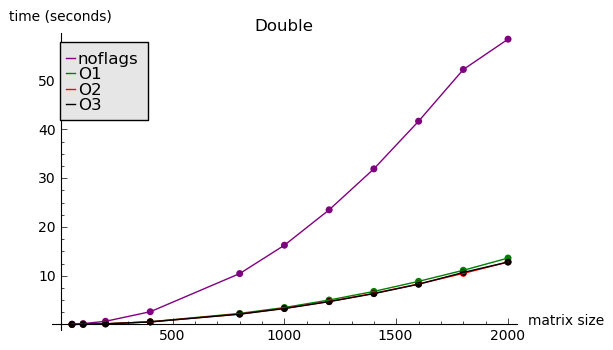
\includegraphics[scale=0.6]{images/double.png}
    \caption{Vector field of equation 2}
\end{figure}


%This is because in the computational kernel, if the current gridpoint is water(value 0), then the code(or program? A better word to repace “code”?) would not do any calculation or upgrade the three 2d arraies(hare, puma and map) as well as we have got that the calculation and upgrading takes the most time by profiling section.

The execution times for different landscape masks can be seen in figure 11. There seems to be a clear correlation between the amount of land (represented by 1's) and the execution time, which is perfectly logical. Nonetheless there was no evidence that the structure of the islands influenced execution time, but more experimentation is needed to determine this (which was not possible to do given the time constraints).


\begin{figure}[hb]
    \centering
    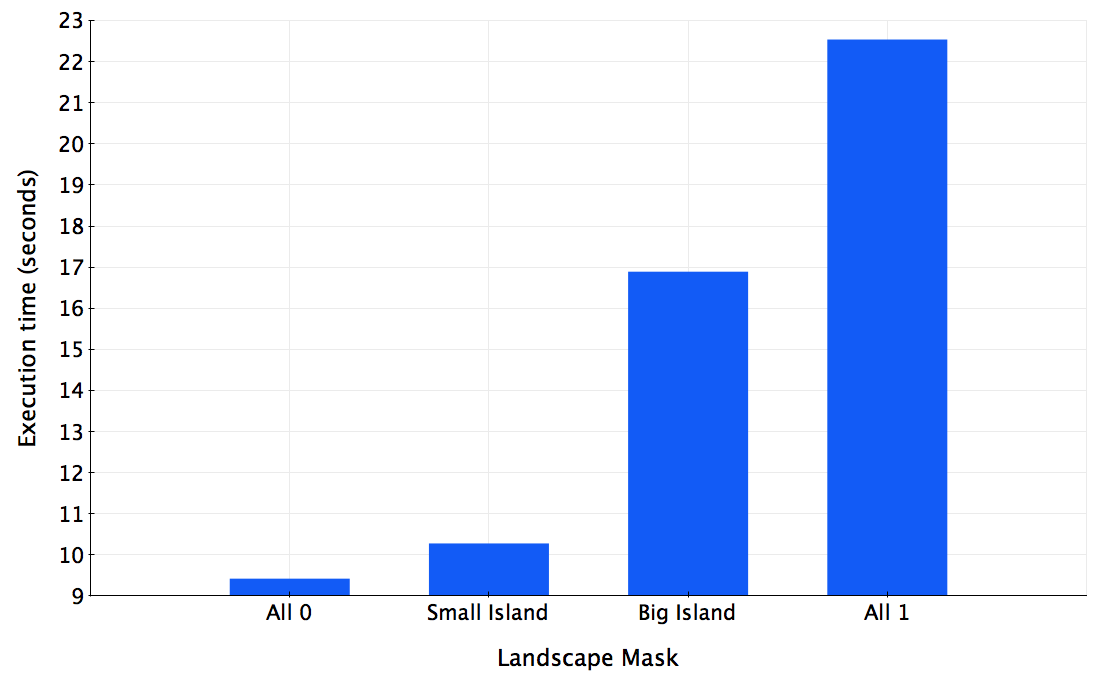
\includegraphics[scale=0.3]{images/bargraph.png}
    \caption{Vector field of equation 2}
\end{figure}


\subsection{Profiling}

GNU GProf was utilized for profiling the software. The compute function (part of the PDE Kernel) takes the majority of execution time. However, the running time of readmap function rises when increasing matrix size. When the input is a $50\times 50$ matrix, the compute function takes $99.99\%$ percent CPU time for the process. When the input is a $2000\times 2000$  matrix, the percentage of time spent in the compute function was reduced significantly. 

This behaviour was actually expected beforehand, but it still tells us that all the optimization efforts must be used in the compute function and disk access should be avoided as much as possible, since this is (by far) the main source of overhead when landscape size is augmented.


%
%%DoubleFlags
%
%\begin{figure}[hb]
%    \centering
%    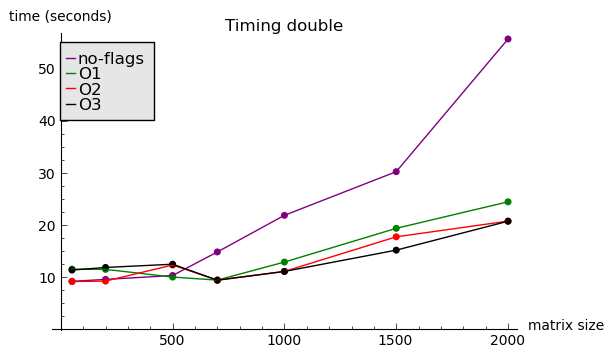
\includegraphics[scale=0.75]{images/DoubleFlags.png}
%    \caption{Vector field of equation 2}
%\end{figure}
%
%
%Figure 9 shows the running time of different optimization options, utilizing double precision. %It is noticeable that with no optimization flags the performance was not only much slower than when utilizing any of the flags, but also the running time increased far more rapidly than in the other cases. The performance between the O1, O2, and O3 was very similar, predictably O3 being the best, although there were no significant 
%
%
%Test 1: different size of landscape	
%
%land/water distribution: random
%
%
%
%
%
%
%Basically, when the matrix size is small the total times are similar (the difference is within 2 seconds)
%
%Obviously, the running times of optimized code increase smoothly and the difference among them is still small. However, the curve without optimization flag increase repidly.
%
%
%
%This is because in the computational kernel, if the current gridpoint is water(value 0), then the code(or program? A better word to repace “code”?) would not do any calculation or upgrade the three 2d arraies(hare, puma and map) as well as we have got that the calculation and upgrading takes the most time by profiling section.


%matrix size: 2000x2000
%			
%input masks:
%
%
%All water
%Small island (a 500x500 island in center)
%Big island (a 1500x1500 island in center)
%All land

\clearpage

\section{Conclusions}

The main objective of this work was to use good software development practices and standards, and see the importance that all stages of the process have, along with producing the best implementation given the time constraints of the project, which was accomplished successfully. 

Working in a team has lots of challenges. Employing good software development processes can improve the quality and efficiency of the project deliverables. We experienced this firsthand while working on this project. By taking a modularized approach to tackle the various tasks in the project, the amount of work was divided as equally as possible. Periodic checkpoints and meetings were essential in order to complete the deliverables on time. The

Coding standards used in the project ensured easy readability and quick detection of bugs within the code, along with easy integration of different components. Code reviews and running stress tests played an important part in making the program robust. The use of a testing framework made the task of unit testing quick and reliable, and also allowed making improvements and optimizations to the code base without breaking the functionality. Also the use of a good revision control system such as Git made the maintenance of the source code simple. Also automating repetitive tasks in the project using scripts improved the overall productivity of the project.
 
One unexpected aspect was the particular importance of automated error testing was particularly important since it  allowed us to realize some aspects of the behaviour that would have otherwise been impossible (at least given the time frame and other projects and course works), like the role of the time step in the convergence algorithm.

The use of performance analysis tools proved very helpful in finding the bottlenecks within the code. A huge performance improvement was achieved by avoiding expensive operations such as copying segments of memory repeatedly in a loop. Use of tools like gdb also was also quite useful in debugging segmentation faults.

By working on this project, every member in the team was able to use the various tools and techniques taught as part of the Programming Skills course, given that some of the main stages of development were shared among all the members.
 




\begin{thebibliography}{100}

%Hoppensteadt, F., "Predator-prey model", Scholarpedia, 1(10), 1563, (2006)

\bibitem{ref:lotka} Hoppensteadt, F., \emph{Predator-prey model}, Scholarpedia, 1(10), 1563, (2006)

\bibitem{ref:sysml} \url{'http://www.sysml.org/specs/'}

%\bibitem{ref:unittest} \emph{http://en.wikipedia.org/wiki/Unit_testing }

\end{thebibliography}


\end{document}

